\documentclass{article}

\usepackage{tikz}

\usepackage{microtype}
\usepackage{parskip}

\title{My Report}
\author{Nick}
\date{\today}

\begin{document}

\maketitle

\begin{figure}[h]
    \centering
    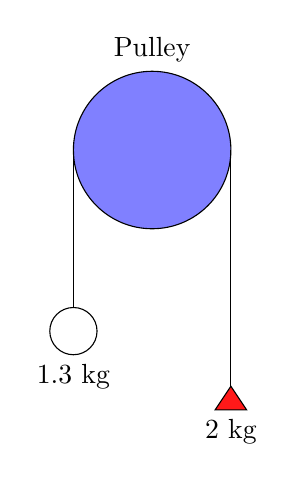
\begin{tikzpicture}
        \filldraw[fill=blue!50] (0,0) circle [radius=1cm];
        \draw (-1,0) -- (-1,-2);
        \draw (1,0) -- (1,-3);
        \filldraw[fill=red!90] (1,-3) -- (1.2,-3.3) -- (0.8,-3.3) -- cycle;
        \draw (-1,-2.3) circle [radius=0.3cm];
        \node [anchor=north] at (1,-3.3) {2 kg};
        \node [anchor=north] at (-1,-2.6) {1.3 kg};
        \node [anchor=south] at (0,1) {Pulley};
    \end{tikzpicture}
    \caption{Setup for the experiment}
\end{figure}

\end{document}